\section{Related Work}

\begin{figure*}[t]
  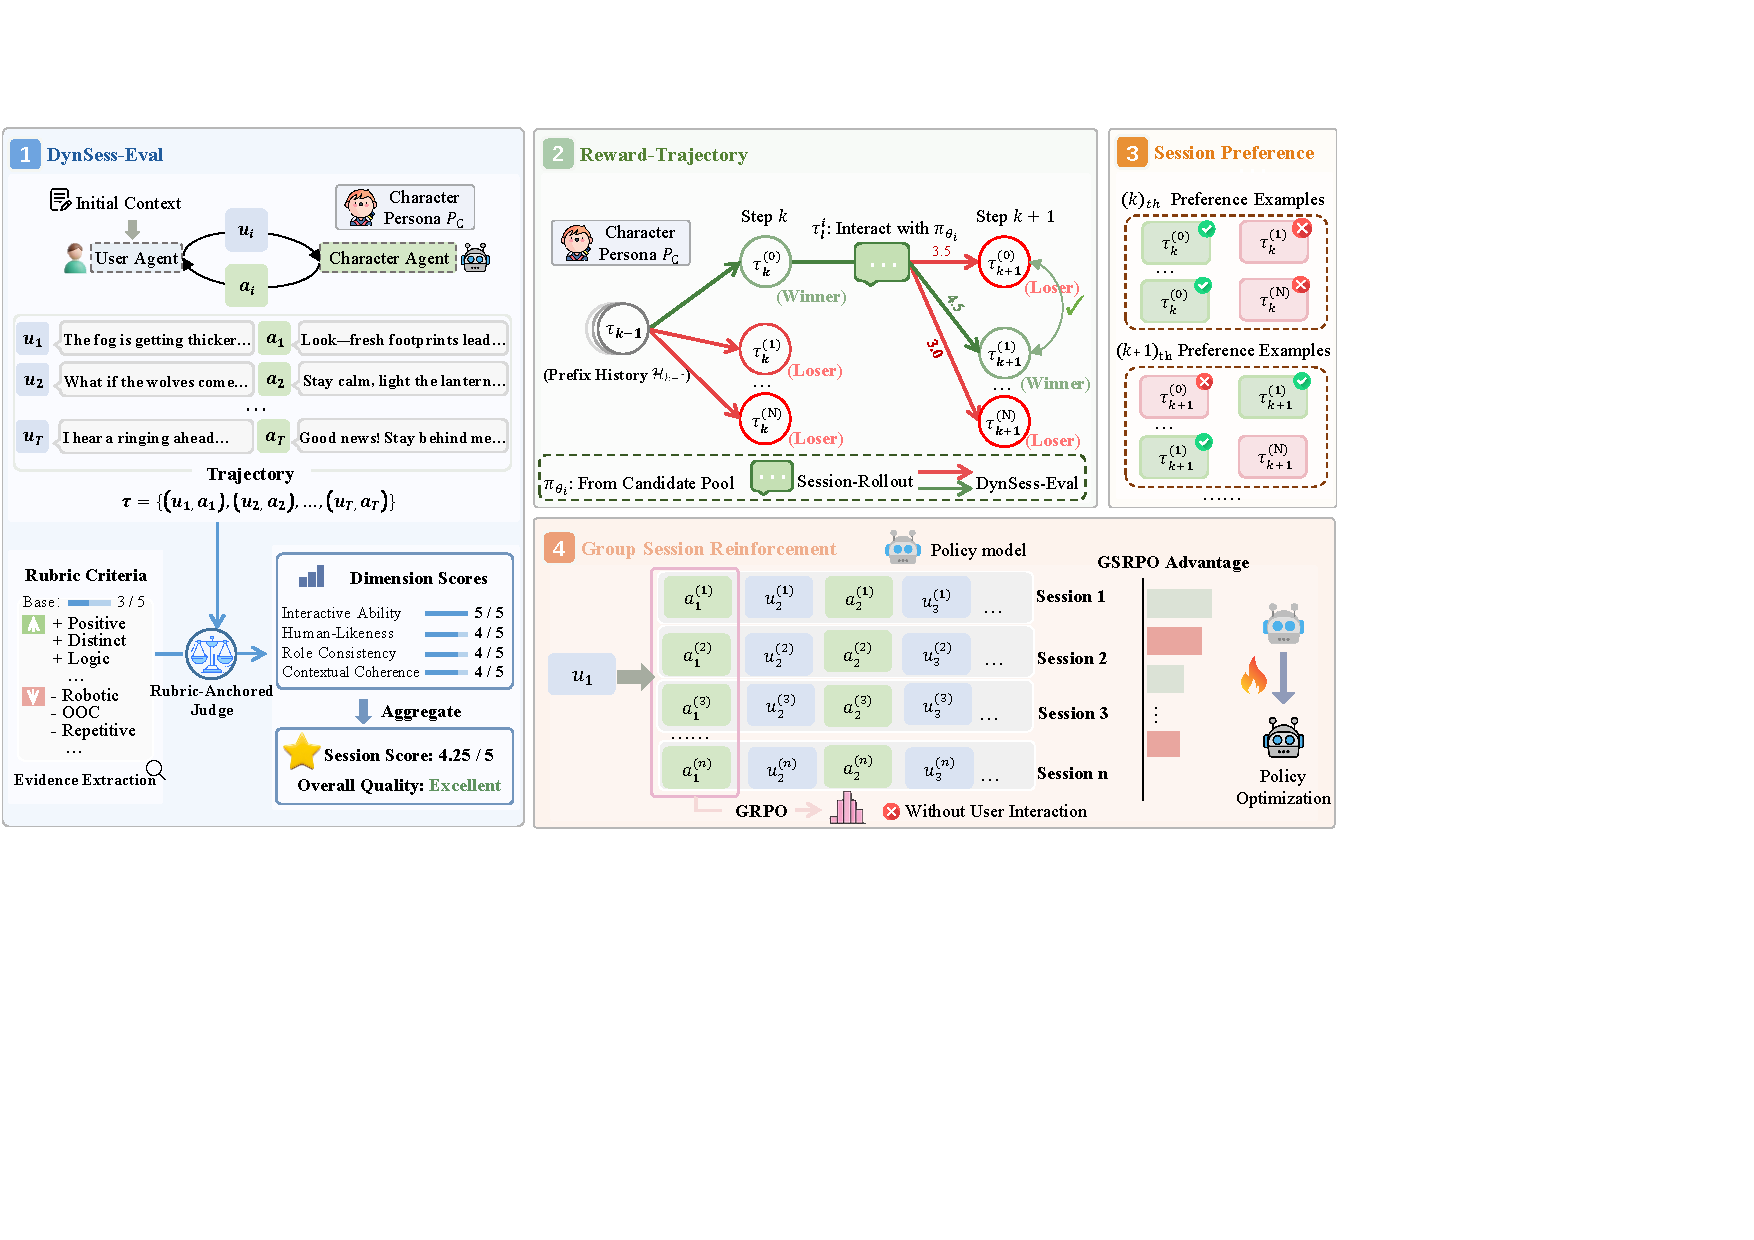
\includegraphics[width=\textwidth,
    trim=0 6.9cm 7cm 2.1cm,
    clip
    ]{latex/Image/method-0526.pdf}
  \caption{Overview of our framework. DynSess-Eval (left) simulates multi-turn user–agent sessions and scores them along four dimensions via a rubric-anchored judge. DynSess-Character (right) leverages these session-level rewards to construct trajectories through multi-turn lookahead search for SFT, and further aligns the agent via off-policy DSPO or on-policy GSRPO.}
  \label{fig:method}
  % \vspace{-0.5cm}
\end{figure*}

\paragraph{LLM-based Role-Playing Agents.}
%zrs
%Early LLM-based role-playing agents mainly relied on prompting to instantiate a target character or speaking style \cite{characterai}. More recent work improves persona fidelity through supervised fine-tuning (SFT) on character-specific dialogue data \cite{do2025aligning, wang-etal-2024-rolellm, zhou-etal-2024-characterglm, zhu-etal-2025-single}. To further reduce out-of-character behavior, recent studies have introduced preference-based alignment methods, including RLHF-style optimization tailored to role-playing settings \cite{ye-etal-2025-cpo, fang2025act}. These approaches have substantially improved response-level persona adherence. However, they are still largely optimized at the turn level, which makes them less well aligned with long-horizon role-playing quality that depends on sustained interaction, evolving emotion, and cross-turn continuity \cite{feng-etal-2025-reasoning}.

%tjj
% Early LLM-based role-playing agents mainly relied on prompting to instantiate a target character \cite{characterai}, while recent work improves persona fidelity via supervised fine-tuning on character-specific dialogues \cite{do2025aligning, wang-etal-2024-rolellm, zhou-etal-2024-characterglm, zhu-etal-2025-single} and preference-based alignment such as RLHF tailored to role-playing \cite{ye-etal-2025-cpo, fang2025act}. Despite improved response-level persona adherence, these methods remain optimized at the turn level and are poorly aligned with long-horizon quality that depends on sustained interaction and cross-turn continuity \cite{feng-etal-2025-reasoning}.

Early LLM-based role-playing agents mainly relied on prompting to instantiate a target character \cite{characterai}, while recent work improves persona fidelity via supervised fine-tuning on character-specific dialogues \cite{do2025aligning, wang-etal-2024-rolellm, zhou-etal-2024-characterglm, zhu-etal-2025-single} and preference-based alignment such as RLHF tailored to role-playing \cite{ye-etal-2025-cpo, fang2025act}. Recent studies further examine the limitations of reasoning-oriented role-playing \cite{feng-etal-2025-reasoning}, evaluate and enhance plot progression with RolePlot \cite{zhang-etal-2025-roleplot}, and combine configurable persona construction, evaluation, and training in Crab \cite{he-etal-2025-crab}. Despite these advances, existing methods do not consistently use dynamically co-produced sessions as the common unit across evaluation, trajectory construction, and policy optimization. DynSess addresses this gap by connecting these stages through a shared session-level reward.

% LLM-based role-playing agents have evolved from prompt engineering \cite{characterai} to supervised fine-tuning (SFT) on character-specific dialogues \cite{do2025aligning, wang-etal-2024-rolellm, zhou-etal-2024-characterglm, zhu-etal-2025-single}. To better align models with specific personas, recent work has shifted toward reinforcement learning from human feedback (RLHF) \cite{ye-etal-2025-cpo, fang2025act}. These preference-based methods reduce out-of-character behaviors by aligning models with persona-specific preferences. However, turn-level optimization constrains these methods to static traits such as vocabulary and tone, resulting in mechanical  responses that capture surface-level characteristics but lack natural emotional progression and narrative initiative \cite{feng-etal-2025-reasoning}.

\paragraph{Evaluation of Role-Playing Agents.}
%zrs
%Role-playing evaluation has also been dominated by response-level judging. Many benchmarks adopt an LLM-as-a-Judge paradigm to score generated outputs against criteria such as persona fidelity, factual consistency, and stylistic matching \cite{wang-etal-2024-rolellm, li2023chatharuhi}. Representative examples include CharacterEval \cite{tu-etal-2024-charactereval}, which evaluates multiple dimensions of character portrayal, and InCharacter \cite{wang-etal-2024-incharacter}, which probes whether a model remains in character under psychologically informed tests. More recent work has begun to move beyond purely static single-turn settings. CharacterBench \cite{DBLP:conf/aaai/ZhouHWBCK0XPTZZ25} uses targeted contexts to test specific capabilities, while other recent benchmarks introduce multi-turn interaction settings. However, existing evaluation protocols still tend to focus on isolated responses, score dialogues turn by turn, or provide only relative preference signals, leaving limited support for interpretable assessment of complete sessions. As a result, current benchmarks provide only partial evidence about long-horizon role-playing abilities such as narrative initiative, emotional progression, and contextual continuity.
Role-playing evaluation has likewise been dominated by response-level judging. Many benchmarks adopt an LLM-as-a-Judge paradigm to score outputs against criteria such as persona fidelity, factual consistency, and stylistic matching \cite{wang-etal-2024-rolellm, li2023chatharuhi}. Representative examples include CharacterEval \cite{tu-etal-2024-charactereval} and InCharacter \cite{wang-etal-2024-incharacter}, the latter probing whether models remain in character under psychologically informed tests. Recent work has begun moving beyond static single-turn settings: CharacterBench \cite{DBLP:conf/aaai/ZhouHWBCK0XPTZZ25} uses targeted contexts to test specific capabilities, and other benchmarks introduce multi-turn interactions. Yet existing protocols still focus on isolated responses, score dialogues turn by turn, or provide only relative preference signals, offering limited evidence about long-horizon abilities such as narrative initiative, emotional progression, and contextual continuity.

% Role-playing fidelity is evaluated using LLM-as-a-Judge frameworks \cite{wang-etal-2024-rolellm, li2023chatharuhi}. Benchmarks like CharacterEval \cite{tu-etal-2024-charactereval}, CharacterBench \cite{DBLP:conf/aaai/ZhouHWBCK0XPTZZ25}, and InCharacter \cite{wang-etal-2024-incharacter} have standardized how we test factual recall and style matching. However, these paradigms evaluate responses in isolation. By scoring static contexts, they miss how characters adapt over time. A model can ace current benchmarks while completely failing at long-term memory, emotional pacing, and narrative progression—precisely the session-level capabilities current benchmarks fail to measure.

\paragraph{Optimization in Multi-Turn Dialogue.}
% zrs
%Beyond role-playing, recent work has explored session-level optimization to better model sequential dependencies in multi-turn interaction \cite{shani2024multi, li2025beyond}. Existing methods for multi-turn RLHF \cite{gao2024regressing, zhou2024archer} and trajectory-level DPO \cite{kong2025sdpo, shi2024direct} typically focus on task-oriented domains where trajectory quality can be grounded in relatively clear terminal rewards, such as task completion or solution correctness. Open-ended role-playing differs in two important ways. First, there is usually no deterministic end-state that defines success. Second, session quality depends on subjective but important properties such as story flow, persona consistency, and interaction naturalness. Constructing useful trajectory-level preference signals for such open-ended sessions therefore remains a central challenge. This challenge motivates our focus on session-level evaluation and preference optimization for role-playing agents.
Beyond role-playing, recent work has explored session-level optimization to capture sequential dependencies in multi-turn interaction \cite{shani2024multi, li2025beyond}. Existing methods for multi-turn RLHF \cite{gao2024regressing, zhou2024archer} and trajectory-level DPO \cite{kong2025sdpo, shi2024direct} typically target task-oriented domains, where trajectory quality can be grounded in clear terminal rewards such as task completion or solution correctness. Open-ended role-playing differs in two key ways: there is no deterministic end-state defining success, and session quality hinges on subjective properties like story flow, persona consistency, and interaction naturalness. Constructing trajectory-level preference signals for such sessions thus remains a central challenge, motivating our focus on session-level evaluation and preference optimization for role-playing agents.

% Recent work explores session-level optimization to capture sequential dependencies in multi-turn dialogues \cite{shani2024multi, li2025beyond}. Current methods for multi-turn RLHF \cite{gao2024regressing, zhou2024archer} and trajectory-level DPO \cite{kong2025sdpo, shi2024direct} target task-oriented domains where terminal rewards are deterministic (e.g., task completion, solution correctness). Open-ended role-playing lacks these clear endpoints. Session quality relies on subjective qualities like story flow and character consistency. Constructing trajectory-level preferences from subjective session quality rather than deterministic rewards remains an open challenge.